\documentclass[../main.tex]{subfiles}

\begin{document}

\section{Probability Theory} \label{probability}
A probability is a measure of how frequent or likely an event will take place. 

    \paragraph{Probability interpretations}
        \begin{itemize}
            \item [] \textbf{Frequentist:} Fraction of positive samples, if we measured infinitely many samples.
            \item [] \textbf{Objectivist:} Probabilities are due to inherent uncertainty properties.
            \item [] \textbf{Subjectivist:} An agent's degree of belief (not external).
            \item [] \textbf{Bayesian:} (Building on subjectivism) A reasonable expectation on the basis of a state of knowledge/evidence.
        \end{itemize}
        \attention Also the frequentist view is subjective since you need to compare events on otherwise similar objects. Usually there are no completely similar objects, so you need to define them. \\
        \btw The Bayesian view allows to give certainties to events, where we don't have samples on (e.g. disappearance of the south pole until 2030).

    \paragraph{Probability Space} \index{Probability Space} The probability space is a triplet space containing a sample/outcome space $\Omega$ (containing all possible atomic events), a collection of events $S$ (containing a subset of $\Omega$ to which we want to assign probabilities) and the mapping $P$ between $\Omega$ and $S$. 

    \paragraph{Axioms of Probability} \index{Axioms of Probability} The mapping $P$ must fulfill the axioms of probability: 
            \begin{enumerate}
                \item $P(a) \geq 0$
                \item $P(\Omega) = 1$
                \item $a,b \in S$ and $a \cap b = \{\}$ $ \Rightarrow P(a \cup b) = P(a) + P(b)$
            \end{enumerate}

    \paragraph{Random Variable (RV)} \index{Random Variable} A RV is a function that maps points from the sample space $\Omega$ to some range (e.g. Real numbers or booleans). They are characterized by their distribution function. E.g. for a dice roll:
            \[ X(\omega) = \begin{cases} 
                0, \text{ if } \omega = heads\\
                1, \text{ if } \omega = tails.
            \end{cases}
            \]

    \paragraph{Proposition} \index{Proposition} A Proposition is a conclusion of a statistical inference that can be true or false (e.g. a classification of a datapoint). More formally: A disjunction of events where the logic model holds. An event can be written as a \textbf{propositional logic model}:\\ $A = true, B = false \Rightarrow a \land \neg b $. Propositions can be continuous, discrete or boolean. 

%%%%%%%%%%%
\subsection{Probability distributions(PDF)} \index{Probability distribution}
        Probability distributions assign probabilities to to all possible points in $\Omega$ (e.g. $P(Weather) = \langle 0.3, 0.4, 0.2, 0.1 \rangle$, representing Rain, sunshine, clouds and snow). 
        Joint probability distributions give you a probability for each atomic event of the RVs (e.g. $P(weather, accident)$ gives you a $2\times 4$  matrix.)

        \paragraph{Cumulative Distribution Function (CDF)} \index{Cumulative Distribution Function} The CDF is defined as $F_X(x) = P(X \leq x)$ (See figure \ref{CDF}).
                \begin{figure}
                    \centering  
                    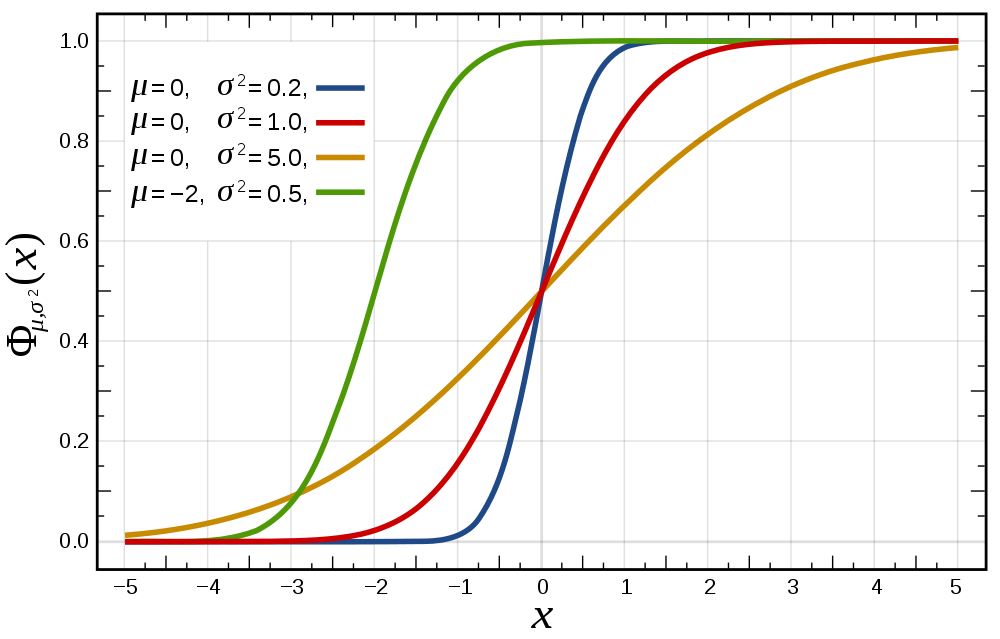
\includegraphics[width=0.6\textwidth]{../figures/Normal_Distribution_CDF.png}
                    \caption{Cumulative distribution function of a normal distribution for different mean ($\mu$) and variance ($\sigma$). \textit{Source: \href{https://commons.wikimedia.org/wiki/File:Normal_Distribution_CDF.svg}{user Inductiveload on wikimedia.org}.}}
                    \label{CDF}
                \end{figure}

        \paragraph{Probability Density Function (PDF)} \index{{Probability Density Function}} For continuous functions the PDF is defined by 
                \begin{equation}
                    p(x) =  {d \over dx} p(X \leq x).
                \end{equation}
                The probability of x being in a finite interval is
                \begin{equation}
                    P(a < X \leq b) = \int_a^b p(x) dx
                \end{equation}
                A PDF is shown in figure
                \begin{figure}
                    \centering
                    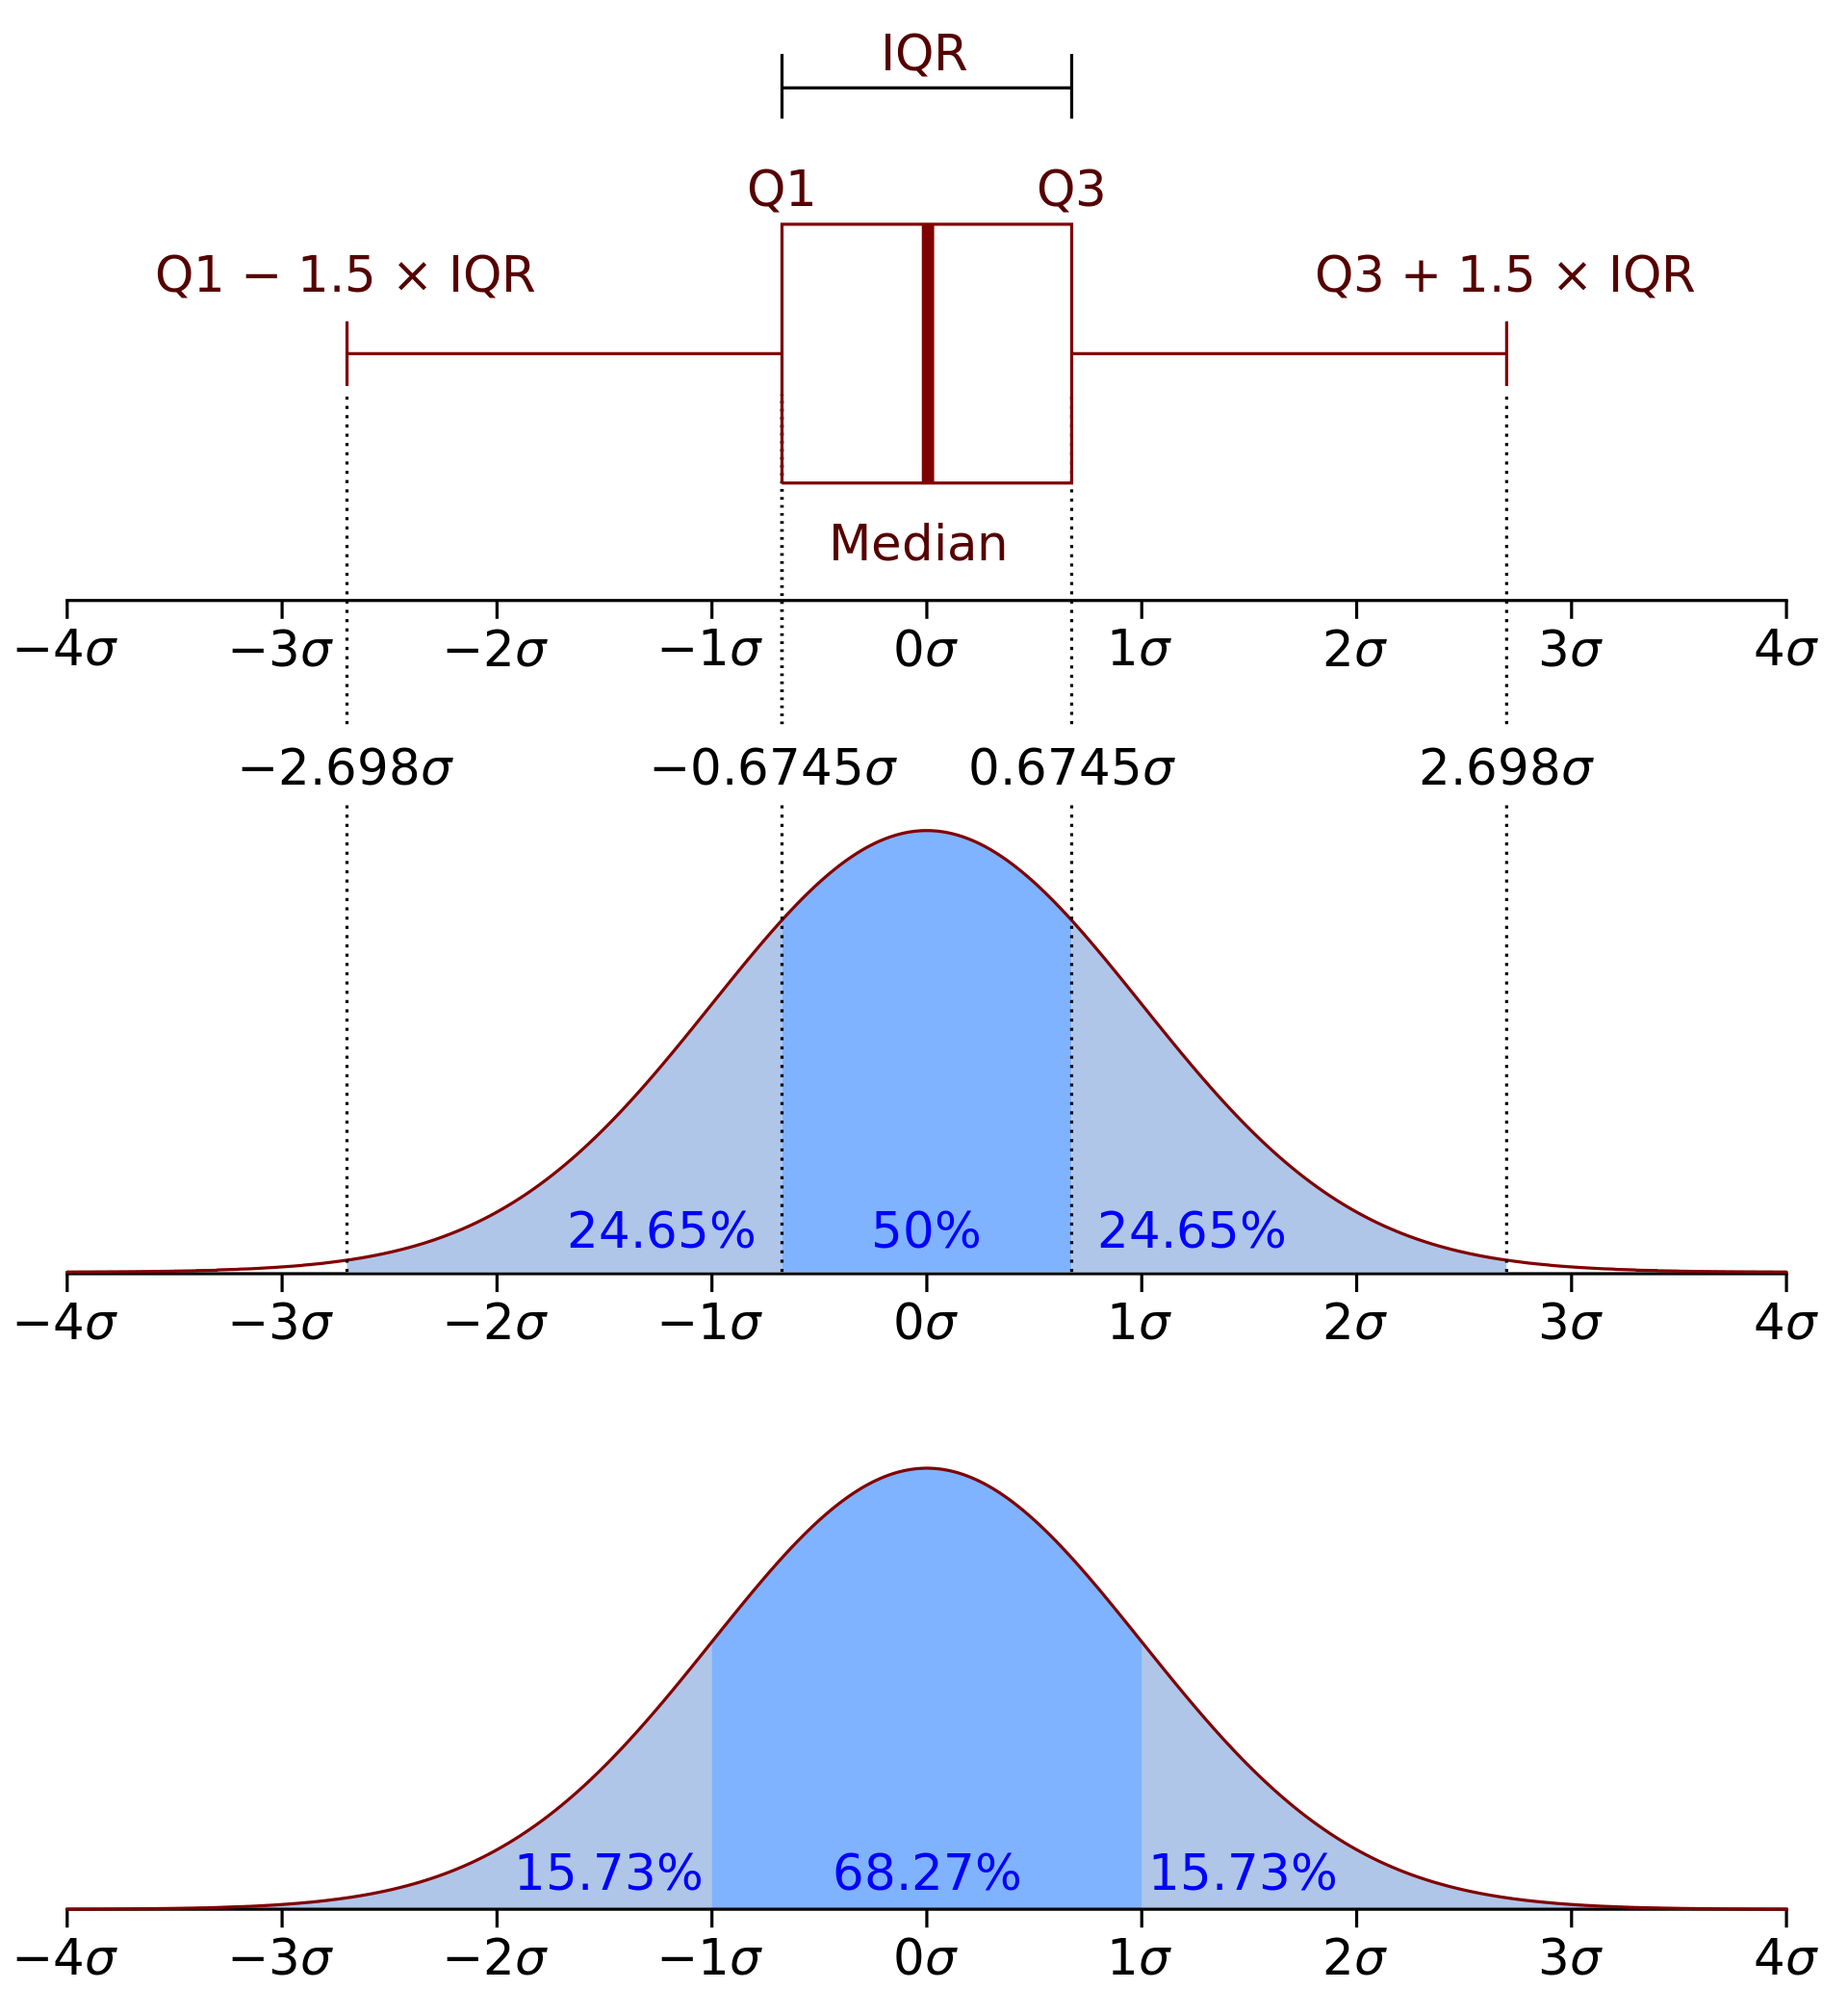
\includegraphics[width=0.6\textwidth]{../figures/Boxplot_vs_PDF.png}
                    \caption{Probability density function of a normal distribution with variance ($\sigma$). In red a range from a Box-plot is shown with quartiles (Q1, Q3) and interquartile range (IQR). For the cutoffs (borders to darker blue regions) the IQR (on top) and $\sigma$ are chosen. Another common cutoff is the confidence interval with light blue regions having a probability mass of $2 * \alpha / 2$. \textit{Source: \href{https://commons.wikimedia.org/wiki/File:Boxplot_vs_PDF.svg}{user Jhguch on wikimedia.org}.}}
                    \label{Boxplot}
                \end{figure}

        \paragraph{Properties of Distributions} 
            \begin{itemize}
                \item[] The \textbf{expected value} \index{expected value} ($E$) or \textbf{mean} ($\mu$) is given by $E[X] = \sum_{x \in X} x*p(x)$ for discrete RVs and $E[X] = \int_X x*p(x) dx$ for continuous RVs.
                \item[] The \textbf{variance} \index{variance} measures the spread of a distribution: $var[X] = \sigma^2 = E[(X-\mu)^2] = E[X]^2 - \mu^2$.
                \item[] The \textbf{standard deviation} \index{standard deviation} is given by: $\sqrt{var[X]} = \sigma$.
                \item[] The \textbf{mode} \index{mode} is the value with the highest probability (or the point in the PDF with the highest value): 
                \item[] The \textbf{median} \index{median} is the point at which all point less than the median and all points greater than the median have the same probability ($0.5$). 
                \item[] The \textbf{quantiles} ($Q$) \index{quantile} divide the datapoints into sets of equal number. The $Q_1$ qua\textbf{r}tile has 25\% of the values below it. 
            \end{itemize}

        \paragraph{Dirac delta function} \index{dirac delta function} \label{diracdelta} is a function that is infinite at one point and 0 everywhere else: $$\delta(x)=\begin{cases} \infty , \text{\hspace{1em} if } x = 0 \\0, \text{\hspace{1em} if } x \neq 0 \end{cases} \text{\hspace{1em} and } \int_{-\infty}^{\infty} \delta(x) dx = 1$$

    \subsubsection{Uniform distribution} \index{Uniform distribution}
            The uniform distribution has the same probability throughout a specific interval:
            % \begin{equation}
            %     \text{Unif}(a,b) = \frac{1}{b-a} \mathbb{I}(a < x \leq b) = 
            % \end{equation}
            \[ \text{Unif}(a,b) = \frac{1}{b-a} \mathbb{1}(a < x \leq b) = \begin{cases} 
                \frac{1}{b-a}, \text{\hspace{1em}if } x \in [ a,b ] \\
                0, \text{\hspace{1em}else}
            \end{cases}
            \]
            $\mathbb{1}$ is a vector of ones. 

    \subsubsection{Discrete distributions}
        Used for random variables that have discrete states.

        \paragraph{Binomial distribution} \index{Binomial distribution} Used for experiments with two outcomes (e.g. coin flips). 
                $$X \sim \text{Bin}(n, \theta ) \text{\hspace{1em},Bin}(k|n,\theta)={n \choose k} \theta^k (1-\theta)^{n-k} \text{\hspace{1em},}\frac{n!}{k!(n-k)!},$$ 
                where $n$ is the number of total experiments, $k$ is the number of sucessful experiments and $\theta$ is the probability of success of an experiment.

        \paragraph{Bernoulli distribution} \index{Bernoulli distribution} Is a special case of the binomial distribution with $n=1$. 
                $$X \sim \text{Ber}(\theta ) \text{\hspace{1em},Ber}(x | \theta)=\theta^{\mathbb{1}(x=1)} (1-\theta)^{\mathbb{1}(x=0)}= \begin{cases}
                    \theta, \hspace{1em}\text{if } x=1 \\
                    1 - \theta, \hspace{1em}\text{if } x=0
                \end{cases} $$

        \paragraph{Multinomial distribution} \index{multinomial distribution} Used for experiments with k different outcomes (e.g. dice rolls).
                $$\text{Mu}(x|n,\theta) =  {n \choose x_1, ..., x_K}\prod_{i=1}^K\theta_j^{x_j} = \frac{n!}{x_1!, ..., x_k!}\prod_{i=1}^K\theta_j^{x_j},$$
                where $k$ is the number of outcomes, $x_j$ is the number times that outcome $j$ happens. $X = (X_1, ..., X_K)$ is the \textit{random vector}. 

        \paragraph{Multinoulli distribution} \index{Multinoulli distribution} Is a special case of the multinomial distribution with $n=1$. The random vector is then represented in \textit{dummy-} or \textit{one-hot-encoding} (e.g. $(0,0,1,0,0,0)$ if outcome 3 takes place).
                $$\text{Mu}(x|1,\theta) = \prod_{j=0}^K \theta_j^{\mathbb{1}(x_j=1)}$$

        \paragraph{Empirical distribution} \index{Empirical distribution} $$\text{p}_{\text{emp}}(A) = \frac{1}{N} \sum_{i=1}^N \delta_{x_i}(A), \text{\hspace{1em}} \delta_{x_i}=\begin{cases}1, \text{\hspace{1em} if } x \in A \\0, \text{\hspace{1em} if } x \notin A \end{cases},$$ w
                where $x_1, ..., x_N$ is a data set with N points. The points can also be weighted: 
                $$p(x) =  \sum_{i=1}^N w_i \delta_{x_i}(x)$$ 


    \subsubsection{Continuous distributions}
        Used for random variables that have continuous states.

        \paragraph{Normal/Gaussian distribution} \index{Normal distribution} \index{Gaussian distribution} Often chosen for random noise because it is simple and needs few assumptions (see sect. \ref{CLT}). The PDF is given by: \label{Normal distribution} \index{Gaussian distribution} $$p(x|\mu\sigma^2)= \frac{1}{\sqrt{2\pi\sigma^2}}\exp\left[-\frac{(x-\mu)^2}{2\sigma^2}\right],$$ where $\mu$ is the mean and $\sigma^2$ is the variance. The CDF is given by: $$\Phi(x) = \frac{1}{\sqrt{2\pi}}\int_{\infty}^xe^{\frac{-t^2}{2}dt}$$

        \paragraph{Multivariate normal/Gaussian distribution} For T datapoints with k dimensions (features). The pdf is:
            $$p(x|\mu,\Sigma) = \dfrac{1}{\sqrt{(2\pi)^k|\Sigma|}}\exp\left[-\dfrac{1}{2}(x-\mu)^\top\Sigma^{-1}(x-\mu)\right], $$  where x now has multiple dimension ($x_1, x_2, ..., x_k$) and $\Sigma$ is the $k \times k$ covariance matrix: $\Sigma = \text{E}[(X-\mu)(X-\mu)]$. The covariance between features is: $\text{Cov}[X_i, X_j] = \text{E}[(X_i-\mu_i)(X_j-\mu_j)]$

        \paragraph{Beta distribution} \index{Beta distribution} defined for $0 \leq x \leq 1$ (see figure \ref{Beta_distr}). The pdf is: $$f(x|\alpha, \beta) = \frac{1}{B(\alpha,\beta)}x^{\alpha-1}(1-x)^{\beta-1}$$ The beta function is there to normalize and ensure that the total probability is 1.
                \begin{figure}
                    \centering
                    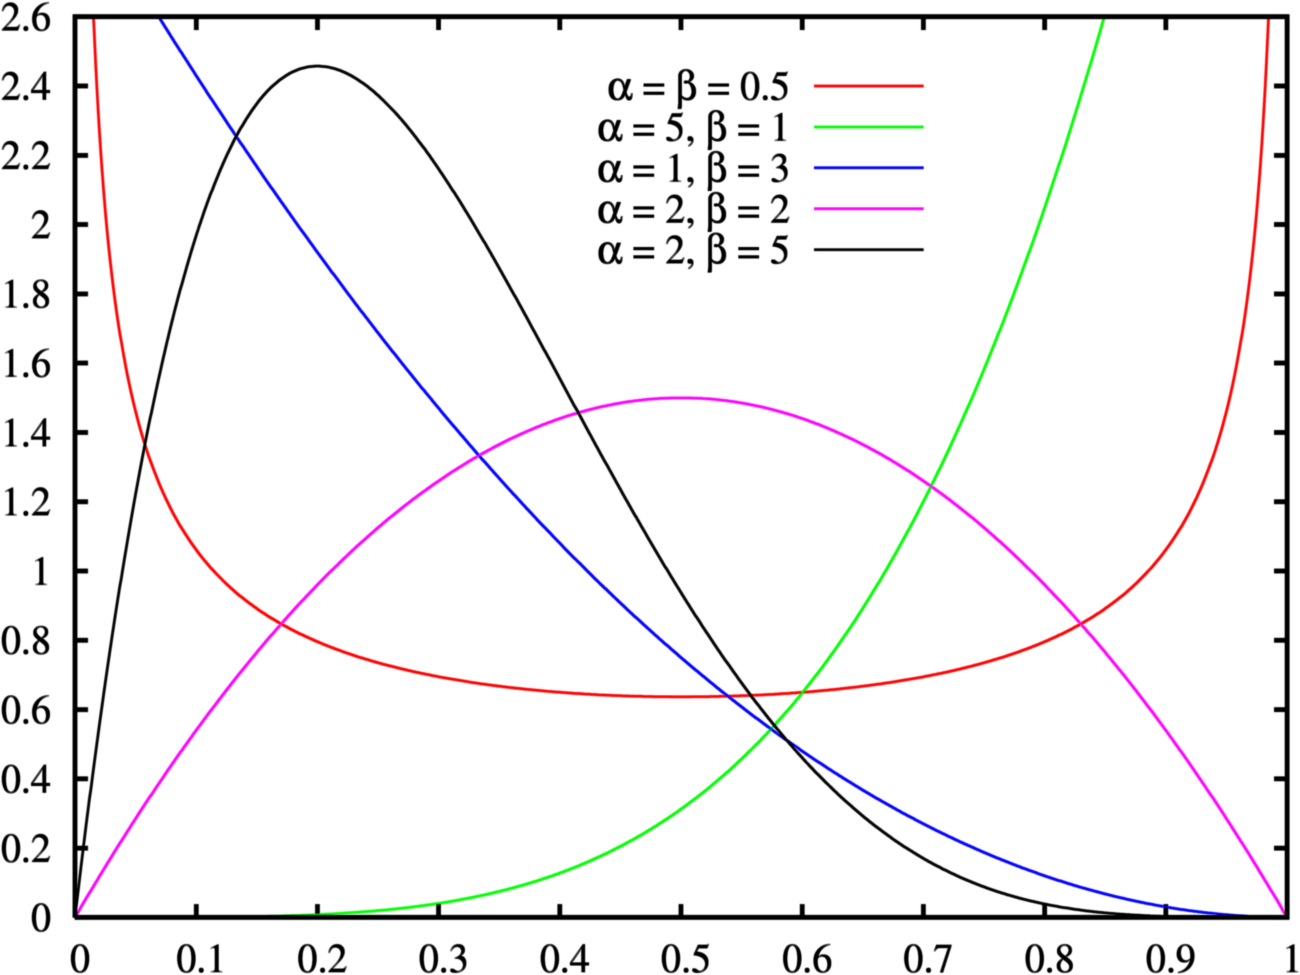
\includegraphics[width=0.6\textwidth]{../figures/Beta_distribution_pdf.png}
                    \caption{Probability density function of a beta-distribution with different parameter values. \textit{Source: \href{https://commons.wikimedia.org/wiki/File:Beta_distribution_pdf.png}{user MarkSweep on wikimedia.org}.}}
                    \label{Beta_distr}
                \end{figure}

        \paragraph{Dirichlet distribution} \index{Dirichlet distribution} The multivariate version of the Beta distribution (see fig. \ref{Dirichlet_distr}). The PDF is: $$\text{Dir}({x}|{\alpha}) \triangleq \dfrac{1}{B({\alpha})}\prod\limits_{i=1}^K x_i^{\alpha_i-1} \text{,\hspace{1em}} \sum_{i=1}^K x_i =1 \text{,\hspace{1em}} x_i \geq 0 \text{ }\forall i$$
                \begin{figure}[h]
                    \centering
                    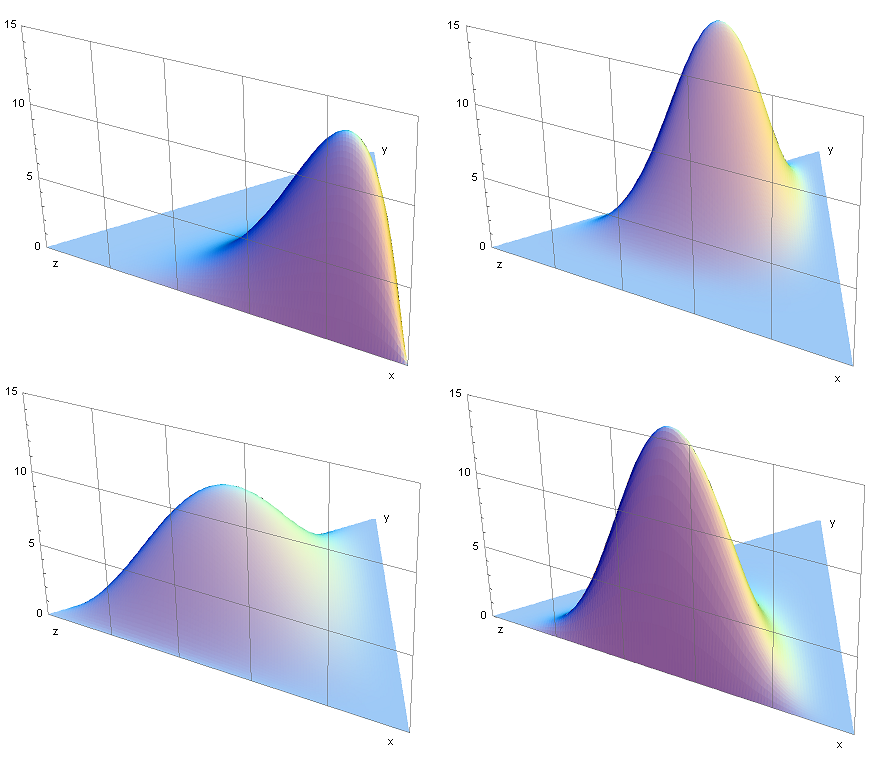
\includegraphics[width=0.6\textwidth]{../figures/Dirichlet_distributions.png}
                    \caption{Probability density function of a Dirichlet-distribution on a 2-simplex (triangle) with different parameter values. Clockwise from top left: $\alpha$ = (6,2,2), (3,7,5), (6,2,6), (2,3,4). \textit{Source: \href{https://commons.wikimedia.org/wiki/File:Dirichlet_distributions.png}{user ThG on wikimedia.org}.}}
                    \label{Dirichlet_distr}
                \end{figure}

        \paragraph{Marginal distributions} \index{Marginal distributions} Are the probability distributions of subsets of the original distribution. Marginal distributions of normal distributions are also normal distributions (see fig. \ref{Multivar_gaussian}).
                \begin{figure}[h]
                    \centering
                    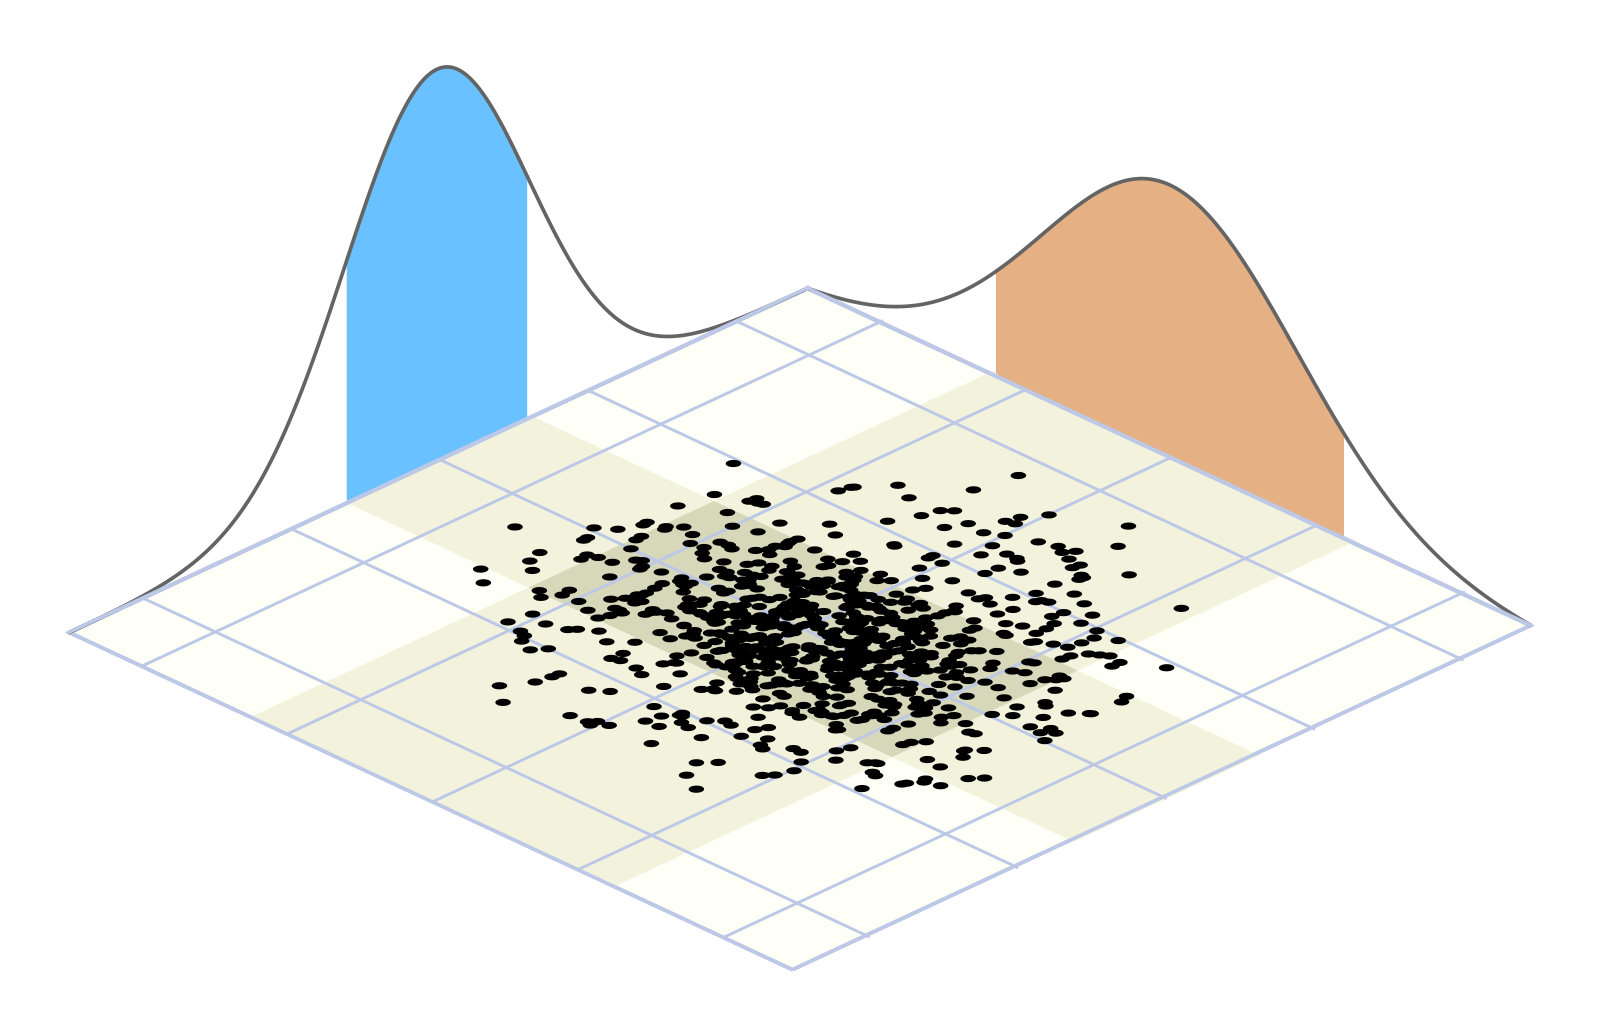
\includegraphics[width=0.6\textwidth]{../figures/Multivariate_gaussian.png}
                    \caption{Data following a 2D-Gaussian distribution. Marginal distributions are shown on the sides in blue and orange. \textit{Source: \href{https://commons.wikimedia.org/wiki/File:Multivariate_Gaussian_inequality_demonstration.svg}{user Auguel on wikimedia.org}.}}
                    \label{Multivar_gaussian}
                \end{figure}


    \subsubsection{Central limit theorem} \index{Central limit theorem} \label{CLT}
    In many cases the sum of random variables will follow a normal distribution as n goes to infinity. 


\subsection{Conditional/Posterior Probability} \index{Conditional probability} \label{posterior}
    Expresses the probability of one event ($Y$) under the condition that another event ($E$) has occurred. (e.g. $C$ = "gets cancer", $S$ = "is a smoker" $\rightarrow$ $p(C|S)=0.2$, meaning: "given the \textit{sole information} that someone is a smoker, their probability of getting cancer is 20\%.") \\
        \\The conditional probability can be calculated like this: 
        $$
        P(A \mid B) = \frac{P(A \cap B)}{P(B)}=\frac{P(A, B)}{P(B)}=\alpha{P(A, B)},
        $$
        where $\alpha$ is used as a normalization constant. If you have hidden variables (confounding factors) you need to sum them out like so:
        $$P(Y|E=e)=\alpha P(Y,E=e)=\alpha\sum_h P(Y,E=e,H=h)$$
        where $X$ contains all variables, $Y$ is called \textit{query variable}, $E$ is called \textit{evidence variable}, $H=X-Y-E$ is called \textit{hidden variable}. You get the joint probabilities by summing out the \\
        \attention Usually $p(A|B) \neq p(B|A)$ \\
        \attention Priors are often forgotten: E.g. $P(\text{"COVID-19"})$ is confused with $P(\text{"COVID-19"}|\text{"Person is getting tested"})$ (because only people with symptoms go to the testing station). \\
        \attention Base rate neglect: Under-representing prior probability. E.g. You have a test with a 5\% false positive rate and a incidence of disease of 2\% in the population. If you are tested positive in a population screening your probability of having the disease is only 29\%. \\
        \btw Conditional distributions of Gaussian distributions are Gaussian distributions themselves.
        
    \paragraph{Independence} \index{Independence} For independent variables it holds: $P(A|B)=P(A)$ or $P(B|A)=P(B)$

    \paragraph{Conditional independence} \index{Conditional independence} Two events $A$ and $B$ are independent, given $C$: $P(A|B,C)=P(A|C)$. $A$ and $B$ must not have any information on each other, given the information on $C$.  E.g. for children: $P(\text{"vocabulary"}|\text{"height"}, \text{"age"})= P(\text{"vocabulary"}|\text{"age"})$.


    \subsubsection{Bayes Rule} \index{Bayes rule}
        \textbf{Bayes rule:} $$ P(\text{hypothesis}|\text{evidence}) =\dfrac{P(\text{evidence}|\text{hypothesis})P(\text{hypothesis})}{P(\text{evidence})}$$
        often used as: 
        $$P(\text{model}|\text{data}) =\dfrac{P(\text{data}|\text{model})P(\text{model})}{P(\text{data})}$$
        
        \paragraph{Terminology:}
        \begin{itemize}
            \item $P(\text{hypothesis}|\text{evidence})$ = Posterior 
            \item $P(\text{evidence}|\text{hypothesis})$ = Likelihood
            \item $P(\text{hypothesis})$ = Prior (How probable hypothesis was before seeing evidence)
            \item $P(\text{evidence})$ = Marginal (How probable evidence is under all possible hypotheses)
            \item $\dfrac{P(\text{evidence}|\text{hypothesis})}{P(\text{evidence})}$ = Support $B$ provides for $A$
            \item $P(\text{data}|\text{model})P(\text{model})$ = joint probability ($P(A,B)$)
            
        \end{itemize}
        \textbf{The proof (see above):} $P(A|B)P(B)=P(A,B)= P(B|A)P(A)$

        \paragraph{Example for Bayes Rule using COVID-19 Diagnostics} $$P(\text{COVID-19}|\text{cough}) =\dfrac{P(\text{cough}|\text{COVID-19})P(\text{COVID-19})}{P(\text{cough})} = \frac{0.7*0.01}{0.1}=0.07$$ Estimating $P(\text{COVID-19}|\text{cough})$ is difficult, because there can be an outbreak and the number changes. However, $P(\text{cough}|\text{COVID-19})$ stays stable, $P(\text{COVID-19})$ and $P(\text{cough})$ can be easily determined.


\subsection{Further Concepts}
        \paragraph{Convergence in Probability of Random Variables} \index{Convergence in probability} You expect your random variables ($X_i$) to converge to an expected random variable $X$. I.e. after looking at infinite samples, the probability that your random variable $X_n$ differs more than a threshold $\epsilon$ from your target $X$ should be zero. 
                $$
                \lim_{n \rightarrow \infty} P(|X_n - X| > \epsilon) = 0
                $$

        \paragraph{Bernoulli's Theorem / Weak Law of Large Numbers} \index{Bernoulli's theorem} \index{Weak law of large numbers} 
                $$
                \lim_{n \rightarrow \infty} P(|\frac{\sum_{i=1}^n X_i}{n} - \mu| > \epsilon) = 0,
                $$
                where $X_1,...,X_n$ are independent \& identically distributed (i.i.d.) RVs. $\Rightarrow$ With enough samples, the sample mean will approach the true mean. The \textbf{strong law of large numbers} \index{strong law of large numbers} states that  $|\frac{\sum_{i=1}^n X_i}{n} - \mu| < \epsilon$ for any $\epsilon > 0$.

        \paragraph{Bias of an estimator} \index{Bias} You have a model with a parameter $\hat{\theta}$ that is an estimator for the true $\theta$. You want to know whether your model over- or underestimates the true $\theta$ systematically. 
                $$
                \text{Bias}[\hat{\theta}]=\text{E}_{X|\mathcal{D}}[\hat{\theta}]- \theta
                $$
        



\end{document}
